% ============================================================
%  第五卷 第五章 费米分布和玻色分布（§53–§63 + 习题）
%  底本：高教社中文版第5版；OCR 底稿 full_merged.md 行 5651–6932
%  插图：图6（§57，p148）、图7（§63，p164）
%
%  已修正的 OCR/原书错误（除注明外均对照原书页面 PNG 核验）：
%   [§53] (53.1)–(53.4) 中花体/粗体记号统一为 \Omega_k、n_k、\varepsilon_k；
%         "当 e^{(μ-σ_k)/T}≪1"之 σ_k→ε_k（p141）；
%   [§54] (54.2) κ_k→ε_k；(54.3) /τ→/T；σ_k→ε_k；
%   [§55] (55.4) 分子分母中 G_j、N_j 上的 OCR 假横线删除（p142 印面无横线）；
%         平衡分布 βε_j（OCR βσ_j）；(55.2)(55.8) \mathrm{ln}→\ln；
%         "熵的表达示如下"断行粘连合并；末句"N_j/G_j."数量级分式还原；
%   [§56] g dτ 中 p_γ→p_y、"dp_*dp_*dp_*"→dp_x dp_y dp_z；
%         (56.4)(56.6)(56.7) /τ、/7→/T；热力学势"𝒂"→Ω；
%         级数展开式 2^{3/2}→2^{5/2}（按 Γ(5/2)/2^{5/2}，p146 印面证实）；
%         "齐次函数"一段按 p146 补"因此"并把 S/V、N/V 两式排为一行
%         （OCR 伪记号 \bar{\mathcal H}≡ 删除，"而"→"和"）；
%         (56.10)(56.11)(61.8) OCR 乱码 \frac{\varkappa}{...}**×→\text{常数}；
%         T^{s/2}→T^{5/2}；(56.15) 3\prime2→3/2；
%         OCR 窜入正文的 E=Nμ+TS-PV=-μ∂Ω/∂μ-T∂Ω/∂T+Ω 一式系 p146 脚注①
%         之文本，按页面删除（脚注文本归脚注代理）；
%   [§57] "对于电子来讲，B=2"→g=2（p147）；p_r、ε_r、T_r→p_F、ε_F、T_F；
%         (57.4) ε^{-μ}→ε-μ；(57.6) (3π²) 补上标 2/3（p148，OCR 丢上标）；
%         习题答案 ν 同样补 1/3（p150）；"对 dp 从 0 积到 p"→p_F；
%         习题解中被 OCR 窜入的脚注①文本（简并化温度 40Z^{4/3}eV≈…）
%         按 p149 页面删除（归脚注代理）；"所求 p_♭"乱码按 p150 还原为
%         "所求的（相对于 1cm^2 器壁的）碰撞次数ν"；
%   [§58] -μτ→-μ/T；推导式中 e'（OCR 乱码）→e^z；
%         f''(μ)→f'''(μ)（两处，p150–151 印面均为三撇）；
%         (58.7) 2γ3、4γ3→2/3、4/3；
%         "把积分上限换成无穷大"后 OCR 乱码 ∇·Φ 为圈码①（p150）；
%         页 151 脚注①（ζ 函数积分公式(1)–(5)及伯努利数、ζ、Γ 值表）系
%         脚注文本，按 p151 页面自正文删除（归脚注代理）；
%   [§59] (59.1) 磁矩记号 OCR "zη"→\mathfrak{M}（p152 印面为花体 𝔐）；
%         "以 μ∓βH 代替 μ"按 p153 还原（OCR "μ 1+ βH"）；
%         "∂Ω₀/∂μ=▽-N"之 ▽ 删除；(59.9) p_*→p_z；n→n+1（OCR "n n+1"）；
%         中间推导式 ∫_{-∞}^{∞}f(x)dx→∫_{-∞}^{μ}f(x)dx（p154 印面）；
%         页 154 脚注①（欧拉-麦克劳林公式(59.10a)及其推导）系脚注文本，
%         按 p154 页面自正文删除（归脚注代理）；
%   [§60] (60.4) μ/T=p_z²/2mT 之"="→"-"；\tilde I_κ→\tilde I_k；
%         "以很高的频率振荡"后 OCR 乱码 𝔇 为圈码①（p157）；
%         磁矩振幅一段之 √[3]7、𝔷ℋ、1/27×1/27 等 OCR 乱码按 p157 印面
%         还原为 𝔐̃、𝔐̄、𝔐̃/𝔐̄∼(μ/βH)^{1/2}；exp(ε-π²T/βH)→exp(-π²T/βH)；
%   [§61] (61.1) "ε= ,cp"→ε=cp；(61.3) (3π²) 补上标 1/3（p157）；
%         "引人"→引入；习题 3 中 V_c→Vc、p_{ΔF}→p_F；习题 1 v=c→v≈c（p158）；
%   [§62] (62.1) (mT) 补上标 3/2（按 (56.5) 与量纲，p160 印面证实）；
%         (62.3) e^{εT}→e^{ε/T}；(62.5) ζ(5/2)（OCR 5(5/2)）；
%         (62.9) 0.0851_{&}→0.0851g（p161）；T^{s/2}→T^{5/2}；
%         "热容在这一点为极大（等于 1.28×(3/2)N）②"按 p161 印面还原括号；
%         ε=0^{D} 之 D 为圈码①（p161）；习题中 N_o→N₀；
%         "因ℏ在 T=T₀+0 时"→"因而在 T=T₀+0 时"（p162）；
%   [§63] (63.2) \tilde n_k→\bar n_k（p163 印面为平均线）；
%         (63.4) hω→ℏω；"普朗克公式"后 OCR 乱码 𝕆 为圈码①（p164）；
%         (63.12) 单位 \frac{8}{s³·K⁴}→g/(s³·K⁴)（p165，g=克）；
%         (63.15) 下标 ν→V；(63.26) \textbf{l}→1；
%   [全章] \mathrm{d} 收紧；\ln、\exp、\sinh、\coth 等函数名统一；
%         \mathrm{e} 作自然对数底；中文标点全角化；断行粘连多处修复；
%         句末缺句号按文意补（如 §57"愈接近于理想气体"、§63"玻色统计法"等）。
%
%  遗留问题：
%   - 脚注已全部转录完毕（共 24 处 \footnote，圈码已删；对照原书 pages300
%     p155/p156/p158/p161/p164–p172/p176/p178–p180/p183 逐一核验）：
%     §53 p155①；§54 p156①；§55 p158①（球盒队列图按 p158 原书照排）；
%     §56 p161①（E=Nμ+TS−PV=…，即排版代理删除的窜入文本）；
%     §57 p164①（简并化温度 40Z^{4/3}eV≈0.5×10^6 Z^{4/3}K，同上窜入文本）；
%     §58 p165①＋p166①（ζ 积分公式(1)–(5)＋伯努利数、ζ、Γ 值表，
%     脚注内公式编号用 \tag{1}–\tag{5} 手工给出，不占节公式计数器）
%     ＋p167①（C_p−C_v∝T^{2n+1}，原书按印面为 2n+1）；§59 p167②、
%     p169①（欧拉-麦克劳林(59.10a)，\tag 手工编号）②③、p170①②；
%     §60 p171①②、p172①；§62 p176①②；§63 p178①、p179①、p180①、p183①②；
%     （§58 第二个脚注＝p166① ζ 公式脚注，正文多处"参看§58第二个脚注"即此）；
%   - §56"正负号的上号/下号"、§62"把((54.3)式中的)求和转换为((56.5)式中的)
%     积分"之双括号、(58.2) 式中不含 g（§58 按电子气 g=2 论）均系原书原貌
%     （p144/p160/p151），照排；
%   - (46.1a)、(43.9)、(45.6)、(52.1)、(40.2)、(40.3)、(40.4)、(40.8)、(24.16)、
%     (35.3)、(56.14) 等跨章引用号照 OCR，未逐条核页面。
% ============================================================
\chapter{费米分布和玻色分布}

\section{费米分布}

如果理想气体的温度（在给定的密度下）足够低，那么玻尔兹曼统计就不再适用而必须建立另一种统计，在这种统计中粒子在各量子态的平均占有数不能假定为很小.

但是，这种统计是随气体（考虑为由 $N$ 个相同粒子所构成的系统）由何种波函数来描述而有所不同的.大家知道，这些波函数相对于任何一对粒子的交换来讲，不是反对称的，就是对称的：前一种情形发生于半整数自旋的粒子，后一种情形发生于整数自旋的粒子.

由反对称波函数来描述的粒子系统遵循泡利原理：不可能有多于一个以上的粒子同时处在每一个量子态中.以这个原理为基础的统计称为费米统计（或费米—狄拉克统计\footnote{这种统计是由费米（E.~Fermi, 1926）对电子提出的，而它同量子力学的联系由狄拉克（P.~A.~M.~Dirac, 1926）所阐明.}）.

类似于我们在§37中所做过的那样，我们把吉布斯分布应用于气体中处于给定量子态的全部粒子的集合；在§37中已经指出，即使在粒子之间存在着交换作用时也是可以这样做的.我们用 $\Omega_k$ 来代表这个粒子系统的热力学势，根据普遍公式(35.3)，我们有：
\begin{equation}
  \Omega_k=-T\ln\sum_{n_k}\Bigl[\exp\Bigl(\frac{\mu-\varepsilon_k}{T}\Bigr)^{n_k}\Bigr],
\end{equation}
因为在第 $k$ 个状态中的 $n_k$ 个粒子的能量就是 $n_k\varepsilon_k$.根据泡利原理，每一个状态的占有数都只可能取 0 或者 1 两个值.因此我们得到：
\begin{equation*}
  \Omega_k=-T\ln\left(1+\exp\frac{\mu-\varepsilon_k}{T}\right).
\end{equation*}

因为系统中的平均粒子数等于热力学势 $\Omega$ 对化学势 $\mu$ 的导数取反号，所以在现在的情形下，我们就得到所求的在第 $k$ 个量子态中的平均粒子数为导数
\begin{equation*}
  \bar{n}_k=-\frac{\partial\Omega_k}{\partial\mu}
  =\frac{\mathrm{e}^{(\mu-\varepsilon_k)/T}}{1+\mathrm{e}^{(\mu-\varepsilon_k)/T}},
\end{equation*}
或者最后写为
\begin{equation}
  \bar{n}_k=\frac{1}{\mathrm{e}^{(\varepsilon_k-\mu)/T}+1}.
\end{equation}
这就是遵循费米统计的理想气体（或简称之为费米气体）的分布函数.正如所预期的，所有的 $\bar{n}_k\ll1$.当 $\mathrm{e}^{(\mu-\varepsilon_k)/T}\ll1$ 时，公式(53.2)当然就过渡到玻尔兹曼分布函数.

费米分布由以下条件归一化
\begin{equation}
  \sum_k\frac{1}{\mathrm{e}^{(\varepsilon_k-\mu)/T}+1}=N,
\end{equation}
式中 $N$ 是气体中的粒子总数.这个等式以隐函数的形式确定化学势为 $T$ 和 $N$ 的函数.

把 $\Omega_k$ 对所有的量子态求和，就得到整个气体的热力学势 $\Omega$
\begin{equation}
  \Omega=-T\sum_k\ln\left(1+\exp\frac{\mu-\varepsilon_k}{T}\right).
\end{equation}

\section{玻色分布}

现在我们来研究由对称波函数描述的粒子所构成的理想气体，这种理想气体所遵循的统计法称为玻色统计法（或玻色—爱因斯坦统计法）\footnote{这种统计是玻色对光量子提出的，后为爱因斯坦所推广.}.

在对称波函数的情形下，量子态的占有数不受任何限制，而可以具有任意的值.分布函数的推导可以像前一节那样来进行，我们写出：
\begin{equation*}
  \Omega_k=-T\ln\sum_{n_k=0}^{\infty}\Bigl(\exp\frac{\mu-\varepsilon_k}{T}\Bigr)^{n_k}.
\end{equation*}
出现在这里的几何级数只有当 $\exp\left(\dfrac{\mu-\varepsilon_k}{T}\right)<1$ 时才是收敛的.因为这个条件对于所有的 $\varepsilon_k$（$\varepsilon_k=0$ 也包括在内）来说都应该成立，所以显然在任何情形下都应该有：
\begin{equation}
  \mu<0.
\end{equation}

关于化学势，应当提醒一下：玻尔兹曼气体的化学势总是取（绝对值很大的）负值；但是费米气体的 $\mu$ 可负可正.

求出几何级数的和，我们得到：
\begin{equation*}
  \Omega_k=T\ln\left(1-\exp\frac{\mu-\varepsilon_k}{T}\right).
\end{equation*}
由此我们求得平均占有数 $\bar{n}_k=-\dfrac{\partial\Omega_k}{\partial\mu}$ 为：
\begin{equation}
  \bar{n}_k=\frac{1}{\mathrm{e}^{(\varepsilon_k-\mu)/T}-1}.
\end{equation}
这就是遵循玻色统计的理想气体（或简称为玻色气体）的分布函数.玻色分布函数与费米分布函数的区别在于分母中 1 前面的符号相反.也像费米分布函数那样，当 $\mathrm{e}^{(\mu-\varepsilon_k)/T}\ll1$ 时，玻色分布函数自然地过渡到玻尔兹曼分布函数.气体中的粒子总数表示为公式
\begin{equation}
  N=\sum_k\frac{1}{\mathrm{e}^{(\varepsilon_k-\mu)/T}-1},
\end{equation}
把 $\Omega_k$ 对所有的量子态求和，就得到整个气体的热力学势 $\Omega$.
\begin{equation}
  \Omega=T\sum_k\ln\left(1-\exp\frac{\mu-\varepsilon_k}{T}\right).
\end{equation}

\section{非平衡的费米气体和玻色气体}

类似于在§40中的那种做法，同样能计算出非平衡费米气体和玻色气体的熵，而从熵为极大值的条件出发又重新得到费米分布函数和玻色分布函数.

在费米情况下，不可能有多于一个以上的粒子处在每个量子态中，但是 $N_j$ 这个数并不小，一般来讲，是与 $G_j$ 这个数同数量级的（这里所有的符号与§40中的符号相同）.

$N_j$ 个相同粒子分布在 $G_j$ 个状态上（每个状态不可多于一个粒子）的可能方式数不是别的，而就是从 $G_j$ 个状态中选取 $N_j$ 个状态的可能方式数，也就是从 $G_j$ 个元素中选取 $N_j$ 个元素的组合数.因此，我们有：
\begin{equation}
  \Delta\varGamma_j=\frac{G_j!}{N_j!\left(G_j-N_j\right)!}.
\end{equation}
把这个表达式取对数，并对(55.1)中三个阶乘的对数都应用公式(40.3)，我们求得：
\begin{equation}
  S=\sum_j\left\{G_j\ln G_j-N_j\ln N_j-\left(G_j-N_j\right)\ln\left(G_j-N_j\right)\right\}.
\end{equation}
再引入量子态的平均占有数 $\bar{n}_j=\dfrac{N_j}{G_j}$，最后我们得到非平衡费米气体的熵的表达式如下：
\begin{equation}
  S=-\sum_jG_j\left[\bar{n}_j\ln\bar{n}_j+\left(1-\bar{n}_j\right)\ln\left(1-\bar{n}_j\right)\right].
\end{equation}

从这个表达式为极大值的条件出发，根据方程式(40.8)很容易求出确定平衡分布的公式为：
\begin{equation*}
  \bar{n}_j=\frac{1}{\mathrm{e}^{\alpha+\beta\varepsilon_j}+1},
\end{equation*}
正如所希望的那样，它是同费米分布一致的.

最后，在玻色统计的情形下，在每个量子态中可以有任意个粒子数，所以统计权重 $\Delta\varGamma_j$ 就是 $N_j$ 个粒子分布在 $G_j$ 个状态上的一切可能方式的数目.这个数目等于\footnote{可以说，问题在于找出把 $N_j$ 个相同的球分配到 $G_j$ 个盒子中去的方式数. 我们把这些球表示成 $N_j$ 个点按次序排列成一个队列的形式；把盒子编号，并假定用 $G_j-1$ 根竖线排列在点的队列中，表示这些盒子间的分界. 例如，下图
\begin{equation*}
  \cdot\;\big|\;\cdot\,\cdot\,\cdot\;\big|\;\big|\;\cdot\,\cdot\,\cdot\,\cdot\;\big|\;\cdot\,\cdot
\end{equation*}
表示 10 个球分配在五个盒子内：第一个盒子内 1 个球，第二个盒子内 3 个球，第三个盒子内 0 个球，第四个盒子内 4 个球，第五个盒子内 2 个球. 在这个队列中（点或竖线所占据的）位置总数是 $G_j+N_j-1$. 我们所求的把球分配到盒子中去的方式数目就是选取 $G_j-1$ 个竖线位置的可能方式的数目，也就是从 $N_j+G_j-1$ 个元素中选取 $G_j-1$ 个元素的组合数，由此就得到在正文中引用的公式.}
\begin{equation}
  \Delta\varGamma_j=\frac{\left(G_j+N_j-1\right)!}{\left(G_j-1\right)!\,N_j!}.
\end{equation}
对这个表达式取对数，同时，与 $G_j+N_j$ 和 $G_j$ 这两个很大的数相比而略去 1，我们得到
\begin{equation}
  S=\sum_j\left\{\left(G_j+N_j\right)\ln\left(G_j+N_j\right)-N_j\ln N_j-G_j\ln G_j\right\}.
\end{equation}
引入平均占有数 $\bar{n}_j$，我们可以把非平衡玻色气体的熵写成形式
\begin{equation}
  S=\sum_jG_j\left[\left(1+\bar{n}_j\right)\ln\left(1+\bar{n}_j\right)-\bar{n}_j\ln\bar{n}_j\right].
\end{equation}

很容易证明：实际上导致玻色分布的就是这个表达式为极大值的条件.

自然，(55.2)和(55.5)这两个熵的公式在 $N_j\ll G_j$ 的极限情形下都过渡到玻尔兹曼公式(40.4). 费米统计和玻色统计的统计权重(55.1)和(55.4)也都过渡到玻尔兹曼表达式(40.2).为此必须设
\begin{equation*}
  G_j!\approx\left(G_j-N_j\right)!G_j^{N_j},\qquad
  \left(G_j+N_j-1\right)!\approx\left(G_j-1\right)!G_j^{N_j}.
\end{equation*}
但是，必须注意到：统计权重的这种过渡意味着在其中忽略掉数量级为 $\dfrac{N_j^2}{G_j}$ 的项，这是不难证明的；一般来讲，这些项本身并不很小，但是在取对数后，这些项在熵中所给出的修正项具有相对较小的数量级 $\dfrac{N_j}{G_j}$.

最后，每个量子态中的粒子数很大（以致 $N_j\gg G_j$，$\bar{n}_j\gg1$）的极限情形是很重要的，我们写出在这种情形下的玻色气体熵的公式.从量子力学中大家知道，这种情形对应于场的经典波动图像.统计权重(55.4)具有形式
\begin{equation}
  \Delta\varGamma_j=\frac{N_j^{G_j-1}}{\left(G_j-1\right)!},
\end{equation}
而熵为
\begin{equation}
  S=\sum_jG_j\ln\frac{\mathrm{e}N_j}{G_j}.
\end{equation}
以后我们在§71中要用到这个公式.

\section{基本粒子的费米气体和玻色气体}

我们来研究由基本粒子（或者在给定条件下可以看成是基本粒子的粒子）构成的气体.以前已经指出，对于通常的原子气体或分子气体来说，根本不需要应用费米分布或玻色分布，因为用玻尔兹曼分布来描述这些气体实际上总是足够精确的.

在这一节中所有推导出来的公式对于费米和玻色这两种分布具有完全类似的形式，差别只在于一个正负号.在后文中，正负号的上号总是对应于费米统计，而下号对应于玻色统计.

基本粒子的能量归结为它的平动动能，平动动能总是准经典的.因此我们有：
\begin{equation}
  \varepsilon=\frac{1}{2m}\left(p_x^2+p_y^2+p_z^2\right),
\end{equation}
而分布函数就像通常那样过渡到在粒子相空间中的分布.同时应该注意到：在一定的动量值下，粒子的状态还取决于它的自旋方向.因此，把分布函数(53.2)或(54.2)乘以
\begin{equation*}
  g\,\mathrm{d}\tau=g\,\frac{\mathrm{d}p_x\,\mathrm{d}p_y\,\mathrm{d}p_z\,\mathrm{d}V}{(2\pi\hbar)^3},
\end{equation*}
就得到了在相空间体积元 $\mathrm{d}p_x\,\mathrm{d}p_y\,\mathrm{d}p_z\,\mathrm{d}V$ 中的粒子数，式中 $g=2s+1$，而 $s$ 是粒子的自旋.于是，粒子数等于
\begin{equation}
  \mathrm{d}N=\frac{g\,\mathrm{d}\tau}{\mathrm{e}^{(\varepsilon-\mu)/T}\pm1}.
\end{equation}
对 $\mathrm{d}V$ 积分（这归结为以气体的总体积 $V$ 来代替 $\mathrm{d}V$），我们得到按粒子动量分量的分布.在动量空间中变换到球坐标，并对角度进行积分，我们就求得按动量绝对值的分布：
\begin{equation}
  \mathrm{d}N_p=\frac{gVp^2\,\mathrm{d}p}{2\pi^2\hbar^3\left(\mathrm{e}^{(\varepsilon-\mu)/T}\pm1\right)}
\end{equation}
（式中 $\varepsilon=\dfrac{p^2}{2m}$），或按能量的分布：
\begin{equation}
  \mathrm{d}N_\varepsilon=\frac{gVm^{3/2}}{\sqrt{2}\,\pi^2\hbar^3}
  \frac{\sqrt{\varepsilon}\,\mathrm{d}\varepsilon}{\mathrm{e}^{(\varepsilon-\mu)/T}\pm1}.
\end{equation}
这两个公式代替了经典的麦克斯韦分布.

把(56.4)对 $\mathrm{d}\varepsilon$ 积分，我们得到气体中的粒子总数：
\begin{equation*}
  N=\frac{gVm^{3/2}}{\sqrt{2}\,\pi^2\hbar^3}\int_0^{\infty}
  \frac{\sqrt{\varepsilon}\,\mathrm{d}\varepsilon}{\mathrm{e}^{(\varepsilon-\mu)/T}\pm1}.
\end{equation*}
引入新的积分变量 $\dfrac{\varepsilon}{T}=z$，我们把上式改写为形式
\begin{equation}
  \frac{N}{V}=\frac{g(mT)^{3/2}}{\sqrt{2}\,\pi^2\hbar^3}\int_0^{\infty}
  \frac{\sqrt{z}\,\mathrm{d}z}{\mathrm{e}^{z-\mu/T}\pm1}.
\end{equation}
这个公式以隐函数的形式确定了气体的化学势 $\mu$ 对温度 $T$ 和密度 $\dfrac{N}{V}$ 的函数关系.

在公式(53.4)，(54.4)中，同样地把求和变换到积分，我们得到热力学势 $\Omega$ 的表达式如下：
\begin{equation*}
  \Omega=\mp\frac{VgTm^{3/2}}{\sqrt{2}\,\pi^2\hbar^3}\int_0^{\infty}
  \sqrt{\varepsilon}\,\ln\left(1\pm\mathrm{e}^{\frac{\mu-\varepsilon}{T}}\right)\mathrm{d}\varepsilon.
\end{equation*}
作分部积分，求得：
\begin{equation}
  \Omega=-\frac{2}{3}\,\frac{gVm^{3/2}}{\sqrt{2}\,\pi^2\hbar^3}
  \int_0^{\infty}\frac{\varepsilon^{3/2}\,\mathrm{d}\varepsilon}{\mathrm{e}^{(\varepsilon-\mu)/T}\pm1}.
\end{equation}
这个表达式同气体的总能量
\begin{equation}
  E=\int_0^{\infty}\varepsilon\,\mathrm{d}N_\varepsilon
  =\frac{gVm^{3/2}}{\sqrt{2}\,\pi^2\hbar^3}
  \int_0^{\infty}\frac{\varepsilon^{3/2}\,\mathrm{d}\varepsilon}{\mathrm{e}^{(\varepsilon-\mu)/T}\pm1}
\end{equation}
只差一个因子 $-\dfrac{2}{3}$.同时注意到 $\Omega=-PV$，我们因此就得到下述关系式：
\begin{equation}
  PV=\frac{2}{3}E.
\end{equation}
因为这个关系式是精确的，所以它在玻尔兹曼气体的极限情形下也应该满足；事实上，我们把玻尔兹曼气体的值 $E=\dfrac{3}{2}NT$ 代入上式，就得到克拉珀龙方程.

在公式(56.6)中作变量代换 $\dfrac{\varepsilon}{T}=z$，我们求得：
\begin{equation}
  \Omega=-PV=VT^{5/2}f\left(\frac{\mu}{T}\right),
\end{equation}
式中 $f$ 是单变量函数，亦即 $\dfrac{\Omega}{V}$ 是 $\mu$ 和 $T$ 的 $\dfrac{5}{2}$ 次齐次函数\footnote{如果按照表达式(56.9)来计算能量
\begin{equation*}
  E=N\mu+TS-PV=-\mu\,\frac{\partial\Omega}{\partial\mu}-T\,\frac{\partial\Omega}{\partial T}+\Omega,
\end{equation*}
那么我们再次得到关系式(56.8).}.

因此
\begin{equation*}
  \frac{S}{V}=-\frac{1}{V}\left(\frac{\partial\Omega}{\partial T}\right)_{V,\mu}
  \qquad\text{和}\qquad
  \frac{N}{V}=-\frac{1}{V}\left(\frac{\partial\Omega}{\partial\mu}\right)_{T,V}
\end{equation*}
是 $\mu$ 和 $T$ 的 $\dfrac{3}{2}$ 次齐次函数，而它们的比值 $\dfrac{S}{N}$ 是零次齐次函数，即 $\dfrac{S}{N}=\varphi\left(\dfrac{\mu}{T}\right)$.由此可以看出：在绝热过程中（$S$=常数），比值 $\dfrac{\mu}{T}$ 保持不变，又因为 $\dfrac{N}{VT^{3/2}}$ 也只是 $\dfrac{\mu}{T}$ 的函数，所以
\begin{equation}
  VT^{3/2}=\text{常数}.
\end{equation}
于是从(56.9)得出
\begin{equation}
  PV^{5/3}=\text{常数},
\end{equation}
而同样地 $T^{5/2}P=$常数.这些等式同通常单原子气体的泊松绝热曲线方程(43.9)是一致的.但是，应当着重指出：公式(56.10)，(56.11)中的幂指数现在同比热的比值没有关系（因为关系式 $\dfrac{c_p}{c_v}=\dfrac{5}{3}$ 和 $c_p-c_v=1$ 不再成立）.

把公式(56.6)改写成如下形式
\begin{equation}
  P=\frac{g\sqrt{2}\,m^{3/2}T^{5/2}}{3\pi^2\hbar^3}
  \int_0^{\infty}\frac{z^{3/2}\,\mathrm{d}z}{\mathrm{e}^{z-\frac{\mu}{T}}\pm1},
\end{equation}
它同公式(56.5)一起以参量形式（参量是 $\mu$）确定气体的物态方程，即 $P$，$V$ 和 $T$ 之间的关系.在玻尔兹曼气体的极限情形下（与此相应的是 $\mathrm{e}^{\frac{\mu}{T}}\ll1$），也可以从这些公式得到克拉珀龙方程，这是理所应当的.我们通过计算证实这一点，同时给出物态方程展开式的一阶修正项.

当 $\mathrm{e}^{\frac{\mu}{T}}\ll1$ 时，我们把(56.12)中的被积式按 $\mathrm{e}^{\frac{\mu}{T}-z}$ 的幂次展开成级数，保留展开式的头两项，我们就得到：
\begin{equation*}
  \int_0^{\infty}\frac{z^{3/2}\,\mathrm{d}z}{\mathrm{e}^{z-\frac{\mu}{T}}\pm1}
  \approx\int_0^{\infty}z^{3/2}\,\mathrm{e}^{\frac{\mu}{T}-z}
  \left(1\mp\mathrm{e}^{\frac{\mu}{T}-z}\right)\mathrm{d}z
  =\frac{3\sqrt{\pi}}{4}\,\mathrm{e}^{\frac{\mu}{T}}
  \left(1\mp\frac{1}{2^{5/2}}\,\mathrm{e}^{\frac{\mu}{T}}\right).
\end{equation*}
以此代入(56.12)，我们有：
\begin{equation*}
  \Omega=-PV=-\frac{gVm^{3/2}T^{5/2}}{(2\pi)^{3/2}\hbar^3}\,
  \mathrm{e}^{\frac{\mu}{T}}\left(1\mp\frac{1}{2^{5/2}}\,\mathrm{e}^{\frac{\mu}{T}}\right).
\end{equation*}
如果只保留展开式的第一项，我们正好得到单原子气体热力学势的玻尔兹曼值（公式(46.1a)）.次一项给出所求的修正项，因此可以写出：
\begin{equation}
  \Omega=\Omega_{\mathrm{B}}\pm\frac{gVm^{3/2}T^{5/2}}{16\pi^{3/2}\hbar^3}\,
  \mathrm{e}^{\frac{2\mu}{T}}.
\end{equation}
但是对所有热力学势用相应的变量来表示的微小增量（参看(24.16)）都是相等的.因此，用 $T$ 和 $V$ 来表示 $\Omega$ 的修正项（借助于玻尔兹曼表达式也可以得到相同精度），我们就直接得到对自由能的修正项：
\begin{equation}
  F=F_{\mathrm{B}}\pm\frac{\pi^{3/2}}{2g}\,\frac{N^2\hbar^3}{VT^{1/2}m^{3/2}}.
\end{equation}
最后，对体积进行微分，我们就得到所求的物态方程：
\begin{equation}
  PV=NT\left[1\pm\frac{\pi^{3/2}}{2g}\,
  \frac{N\hbar^3}{V(mT)^{3/2}}\right].
\end{equation}
在这个公式中修正项很小的条件同玻尔兹曼统计能够适用的条件(45.6)自然是一致的.因此，我们看到：理想气体的性质偏离经典性质，在给定的密度下降低温度时（或是说，当理想气体开始简并化时）发生，使得在费米统计中压强比它在通常气体中的值有所增加；可以说，在这种情形中，量子力学的交换效应使得粒子之间出现某种附加的有效“排斥力”.

在玻色统计中，气体的压强值向相反的方面偏离——偏向比经典值小的方面；可以说，在这里粒子之间出现了某种附加的有效“吸引力”.

\section{简并电子气}

在足够低的温度下研究费米气体的性质有着非常重要的原则性的意义.在下面我们将看到，这里所指的低温，实际上从别的观点看来可能还是很高的.

下面我们来讨论电子气，因为考虑到它是费米统计最重要的应用.对于电子来讲，$g=2$（自旋 $S=\dfrac{1}{2}$）.

我们从研究绝对零度下的电子气（完全简并化的费米气体）开始.在这种气体中电子按不同量子态的分布方式是使得气体的总能量具有最小的可能值.因为每个量子态不可能有一个以上的电子，所以电子占满了能量从最小值（等于 0）到某个最大值为止的全部状态，这个最大值取决于气体中的电子数.

考虑能级的二重自旋简并（$g=2$），动量绝对值位于间隔 $p$ 和 $p+\mathrm{d}p$ 之间的在体积 $V$ 内运动的电子的量子态数等于
\begin{equation}
  2\,\frac{4\pi p^2\mathrm{d}p\cdot V}{(2\pi\hbar)^3}
  =V\frac{p^2\mathrm{d}p}{\pi^2\hbar^3}.
\end{equation}
电子占据了动量从零到边界值 $p=p_F$ 的全部状态；这个值称为动量空间中的费米球半径.在这些状态中的电子总数为
\begin{equation*}
  N=\frac{V}{\pi^2\hbar^3}\int_0^{p_F}p^2\,\mathrm{d}p
  =\frac{Vp_F^3}{3\pi^2\hbar^3},
\end{equation*}
由此得边界动量
\begin{equation}
  p_F=(3\pi^2)^{1/3}\left(\frac{N}{V}\right)^{1/3}\hbar,
\end{equation}
并且边界能量为
\begin{equation}
  \varepsilon_F=\frac{p_F^2}{2m}=(3\pi^2)^{2/3}\frac{\hbar^2}{2m}
  \left(\frac{N}{V}\right)^{2/3}.
\end{equation}
这个能量具有简单的热力学意义.根据前面的叙述，量子态（具有确定的动量值 $p$ 和自旋投影）的费米分布函数
\begin{equation}
  \bar{n}_p=\frac{1}{\mathrm{e}^{(\varepsilon-\mu)/T}+1}
\end{equation}
在 $T\to0$ 的极限下变为“阶跃”函数：在 $\varepsilon<\mu$ 时为 1，在 $\varepsilon>\mu$ 时为 0（在图6中用实线表示这个函数）.由此可见，在 $T=0$ 时，气体的化学势与电子的边界能量是一致的.
\begin{equation}
  \mu=\varepsilon_F.
\end{equation}

\par\nopagebreak\noindent\begin{minipage}{\linewidth}\centering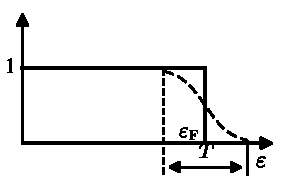
\includegraphics[width=6cm]{fig6.pdf}\\[0.3em]{\small 图 6}\end{minipage}\par\nopagebreak

把状态数(57.1)乘以 $\dfrac{p^2}{2m}$，并遍及所有的动量值进行积分，就得到气体的总能量：
\begin{equation*}
  E=\frac{V}{2m\pi^2\hbar^3}\int_0^{p_F}p^4\,\mathrm{d}p
  =\frac{Vp_F^5}{10m\pi^2\hbar^3},
\end{equation*}
把(57.2)代入上式后得到：
\begin{equation}
  E=\frac{3\left(3\pi^2\right)^{2/3}}{10}\,\frac{\hbar^2}{m}
  \left(\frac{N}{V}\right)^{2/3}N.
\end{equation}
最后，按照普遍关系式(56.8)我们求得气体的物态方程
\begin{equation}
  P=\frac{\left(3\pi^2\right)^{2/3}}{5}\,\frac{\hbar^2}{m}
  \left(\frac{N}{V}\right)^{5/3}.
\end{equation}
由此可见，在绝对零度的温度下，费米气体的压强与密度的 $\dfrac{5}{3}$ 次方成正比.

在给定的气体密度下，所得到的公式(57.6)，(57.7)也可以近似地适用于非常接近绝对零度的温度.显然，这些公式适用（气体为“强简并化”）的条件要求 $T$ 比边界能量 $\varepsilon_F$ 小得多：
\begin{equation}
  T\ll\frac{\hbar^2}{m}\left(\frac{N}{V}\right)^{2/3}.
\end{equation}
正如预期的那样，这个条件与玻尔兹曼统计的适用条件(45.6)是相反的.由关系式 $T_F\approx\varepsilon_F$ 所决定的温度称为简并化温度.

简并电子气具有独特的特性——它的密度愈大，它就愈接近于理想气体.这点容易证实如下.

我们来考虑由电子和带正电荷的原子核所构成的气体，原子核的数量正好能够中和所有电子的电荷.（显然，仅由电子构成的气体是根本不稳定的；我们在前面没有提到原子核，这是由于假设了气体的理想性，因而原子核的存在并不影响电子气的热力学量.）电子同原子核的库仑相互作用能（相对于一个电子来讲）的数量级为 $\dfrac{Ze^2}{a}$，其中 $Ze$ 是原子核的电荷，而 $a\sim\left(\dfrac{ZV}{N}\right)^{1/3}$ 是电子和原子核之间的平均距离.气体理想性的条件归结为要求这个库仑相互作用能远小于电子的平均动能，后者与费米能量 $\varepsilon_F$ 同一数量级.不等式
\begin{equation*}
  \frac{Ze^2}{a}\ll\varepsilon_F,
\end{equation*}
在把 $a\sim\left(\dfrac{ZV}{N}\right)^{1/3}$ 和 $\varepsilon_F$ 的表达式(57.3)代入后，给出条件
\begin{equation}
  \frac{N}{V}\gg\left(\frac{e^2m}{\hbar^2}\right)^3Z^2.
\end{equation}
我们看到：气体密度 $\dfrac{N}{V}$ 愈大，这个条件就满足得愈好\footnote{在电子气密度等于 $\left(\dfrac{e^2m}{\hbar^2}\right)^3 Z^2$ 时，相应的简并化温度是 $40Z^{4/3}\,\mathrm{eV}\approx 0.5\times10^6\,Z^{4/3}\,\mathrm{K}$.}.

\begin{xiti}

\noindent{\heiti 习题}\quad 试求在绝对零度下的电子气中同器壁碰撞的次数.

解：动量大小在间隔 $\mathrm{d}p$ 内而动量方向与器壁法线所成角度在间隔 $\mathrm{d}\theta$ 内的电子数（在单位体积内）为
\begin{equation*}
  \frac{2\cdot2\pi\sin\theta\,\mathrm{d}\theta\,p^2\,\mathrm{d}p}{(2\pi\hbar)^3}.
\end{equation*}
把它乘以 $v\cos\theta$（$v=\dfrac{p}{m}$），并对 $\mathrm{d}\theta$ 从 0 积到 $\dfrac{\pi}{2}$ 且对 $\mathrm{d}p$ 从 0 积到 $p_F$，就得到所求的（相对于 $1\,\mathrm{cm}^2$ 器壁的）碰撞次数 $\nu$.结果求得：
\begin{equation*}
  \nu=\frac{3\left(3\pi^2\right)^{1/3}}{16}\,\frac{\hbar}{m}
  \left(\frac{N}{V}\right)^{4/3}.
\end{equation*}

\end{xiti}

\section{简并电子气的热容}

当温度比简并化温度 $T_F$ 低得多时，分布函数(57.4)具有图6中虚线所示的形式：分布函数只在能量 $\varepsilon$ 的值靠近边界能量 $\varepsilon_F$ 的狭窄间隔内才显著地不等于 1 或 0.这个间隔称为费米分布的展布区，其宽度的数量级为 $T$.

表达式(57.6)，(57.7)为相应量按微小比值 $T/T_F$ 的幂次展开的头一项.我们来确定这些展开式中其次几项.

在公式(56.6)中出现形式为
\begin{equation*}
  I=\int_0^{\infty}\frac{f(\varepsilon)\,\mathrm{d}\varepsilon}{\mathrm{e}^{(\varepsilon-\mu)/T}+1}
\end{equation*}
的积分，式中 $f(\varepsilon)$ 是（使得积分收敛的）某个函数；在(56.6)中，$f(\varepsilon)=\varepsilon^{3/2}$.作代换 $\varepsilon-\mu=Tz$，把这个积分变为：
\begin{equation*}
  I=\int_{-\mu/T}^{\infty}\frac{f(\mu+Tz)}{\mathrm{e}^z+1}\,T\mathrm{d}z
  =T\int_0^{\mu/T}\frac{f(\mu-Tz)\,\mathrm{d}z}{\mathrm{e}^{-z}+1}
  +T\int_0^{\infty}\frac{f(\mu+Tz)\,\mathrm{d}z}{\mathrm{e}^z+1}.
\end{equation*}
在第一个积分中利用
\begin{equation*}
  \frac{1}{\mathrm{e}^{-z}+1}=1-\frac{1}{\mathrm{e}^z+1}
\end{equation*}
就得到：
\begin{equation*}
  I=\int_0^{\mu}f(\varepsilon)\,\mathrm{d}\varepsilon
  -T\int_0^{\mu/T}\frac{f(\mu-Tz)\,\mathrm{d}z}{\mathrm{e}^z+1}
  +T\int_0^{\infty}\frac{f(\mu+Tz)\,\mathrm{d}z}{\mathrm{e}^z+1}.
\end{equation*}
在第二个积分中，我们注意到 $\dfrac{\mu}{T}\gg1$ 而积分收敛得很快，所以把积分上限换成无穷大\footnote{这个替换意味着忽略掉指数型的小项.必须注意，下面得到的展开式(58.1)是渐近的（而并非收敛的）级数.}.因此，我们得到：
\begin{equation*}
  I=\int_0^{\mu}f(\varepsilon)\,\mathrm{d}\varepsilon
  +T\int_0^{\infty}\frac{f(\mu+Tz)-f(\mu-Tz)}{\mathrm{e}^z+1}\,\mathrm{d}z.
\end{equation*}
现在我们把第二个积分中被积式的分子按 $z$ 的幂次展开成泰勒级数，并逐项进行积分：
\begin{equation*}
  I=\int_0^{\infty}f(\varepsilon)\,\mathrm{d}\varepsilon
  +2T^2f'(\mu)\int_0^{\infty}\frac{z\,\mathrm{d}z}{\mathrm{e}^z+1}
  +\frac{1}{3}T^4f'''(\mu)\int_0^{\infty}\frac{z^3\,\mathrm{d}z}{\mathrm{e}^z+1}+\cdots
\end{equation*}
把各个积分的值\footnote{这种类型的积分计算如下：
\begin{equation*}
\begin{aligned}
  \int_0^\infty\frac{z^{x-1}\,\mathrm{d}z}{\mathrm{e}^z+1}
  &=\int_0^\infty z^{x-1}\mathrm{e}^{-z}\sum_{n=0}^\infty(-1)^n\mathrm{e}^{-nz}\,\mathrm{d}z
  =\Gamma(x)\sum_{n=1}^\infty(-1)^{n+1}\frac{1}{n^x}\\
  &=(1-2^{1-x})\,\Gamma(x)\sum_{n=1}^\infty\frac{1}{n^x},
\end{aligned}
\end{equation*}
或
\begin{equation*}
  \int_0^\infty\frac{z^{x-1}\,\mathrm{d}z}{\mathrm{e}^z+1}
  =(1-2^{1-x})\,\Gamma(x)\zeta(x)\qquad(x>0),
\tag{1}
\end{equation*}
式中
\begin{equation*}
  \zeta(x)=\sum_{n=1}^\infty\frac{1}{n^x}
\end{equation*}
是黎曼 $\zeta$ 函数.
当 $x=1$ 时，(1)式变为不定的；积分值为
\begin{equation*}
  \int_0^\infty\frac{\mathrm{d}z}{\mathrm{e}^z+1}=\ln 2.
\tag{2}
\end{equation*}
当 $x$ 为偶数（$x=2n$）时，$\zeta$ 函数可以用所谓伯努利数 $B_n$ 来表示，因而得到：
\begin{equation*}
  \int_0^\infty\frac{z^{2n-1}\,\mathrm{d}z}{\mathrm{e}^z+1}
  =\frac{2^{2n-1}-1}{2n}\,\pi^{2n}B_n.
\tag{3}
\end{equation*}
类似的方式可以用来计算下述积分：
\begin{equation*}
  \int_0^\infty\frac{z^{x-1}\,\mathrm{d}z}{\mathrm{e}^z-1}
  =\Gamma(x)\zeta(x)\qquad(x>1).
\tag{4}
\end{equation*}
当 $x$ 为偶数 $2n$ 时，有：
\begin{equation*}
  \int_0^\infty\frac{z^{2n-1}\,\mathrm{d}z}{\mathrm{e}^z-1}
  =\frac{(2\pi)^{2n}B_n}{4n}.
\tag{5}
\end{equation*}
为了参考起见，我们列出头几个伯努利数的值以及 $\zeta$ 函数和 $\Gamma$ 函数的一些值：
$B_1=\dfrac{1}{6}$，\quad$B_2=\dfrac{1}{30}$，\quad$B_3=\dfrac{1}{42}$，\quad$B_4=\dfrac{1}{30}$；

$\zeta(3/2)=2.612$，\quad$\zeta(5/2)=1.341$，\quad$\zeta(3)=1.202$，\quad$\zeta(5)=1.037$；

$\Gamma(3/2)=\sqrt{\pi}/2$，\quad$\Gamma(5/2)=3\sqrt{\pi}/4$.}代入上式，最后我们有：
\begin{equation}
  I=\int_0^{\mu}f(\varepsilon)\,\mathrm{d}\varepsilon
  +\frac{\pi^2}{6}T^2f'(\mu)+\frac{7\pi^4}{360}T^4f'''(\mu)+\cdots
\end{equation}
展开式的第三项列出供参考，我们在这里并不需要.

在公式(58.1)中令 $f=\varepsilon^{3/2}$ 并将它代入(56.6)，就得到所求的热力学势 $\Omega$ 在低温下的展开式中次一项：
\begin{equation}
  \Omega=\Omega_0-VT^2\frac{\sqrt{2\mu}\,m^{3/2}}{6\hbar^3}.
\end{equation}
$\Omega_0$ 代表 $\Omega$ 在绝对零度下的值.

把第二项看作是对 $\Omega_0$ 的微小增量，并借助于“零级近似”(57.5)把其中的 $\mu$ 用 $T$ 和 $V$ 来表示，可以直接写出自由能的表达式（根据小增量定理(24.16)）
\begin{equation}
  F=F_0-\frac{\beta}{2}NT^2\left(\frac{V}{N}\right)^{2/3},
\end{equation}
式中为了简便起见引入符号
\begin{equation}
  \beta=\left(\frac{\pi}{3}\right)^{2/3}\frac{m}{\hbar^2}.
\end{equation}
由此我们求得气体的熵：
\begin{equation}
  S=\beta NT\left(\frac{V}{N}\right)^{2/3},
\end{equation}
气体热容\footnote{我们不写出热容的角标 $v$ 或 $p$，因为在这种近似下 $C_v$ 和 $C_p$ 是同一的. 的确，我们在§23中已经看到：如果 $T\to0$ 时 $S$ 以 $T^n$ 的方式趋于 0，那么差值 $C_p-C_v$ 依 $T^{2n+1}$ 的方式趋向于 0；因而在这里所考虑的情形下，
\begin{equation*}
  C_p-C_v\propto T^3.
\end{equation*}}
\begin{equation}
  C=\beta NT\left(\frac{V}{N}\right)^{2/3}
\end{equation}
以及能量
\begin{equation}
  E=E_0+\frac{\beta}{2}NT^2\left(\frac{V}{N}\right)^{2/3}
  =E_0\left[1+0.18\left(\frac{mT}{\hbar^2}\right)^2\left(\frac{V}{N}\right)^{4/3}\right].
\end{equation}
由此可见，在低温下简并费米气体的热容与温度的一次方成正比.

\section{电子气的磁性.弱场}

弱磁场中电子气的磁化强度由两个独立部分组成：与电子（自旋的）内禀磁矩有关的顺磁性（泡利顺磁性，W.~Pauli，1927）以及与电子在磁场中的轨道运动量子化有关的抗磁性（朗道抗磁性，L.~D.~Landau，1930）. 设气体是简并化的：温度 $T\ll\varepsilon_F$，我们来计算相应的磁化率.磁场很弱的条件表明：应该有（参看下面）$\beta H\ll T$，式中 $\beta=\dfrac{|e|\hbar}{2mc}$ 是玻尔磁子\footnote{在高温（$T\gg\varepsilon_F$）的相反情况下，电子形成玻尔兹曼气体，单位体积磁化率的顺磁性部分为：$\chi_{\mathrm{para}}=\dfrac{N\beta^2}{VT}$（$g=2$，$J=\dfrac{1}{2}$ 下的公式(52.8)）.}.

对于简并气体，以 $T,V,\mu$（而不是 $T,V,N$）为独立变量进行热力学计算较方便.与此相应，玻尔兹曼气体的磁矩计算公式(52.1)在这里替代为热力学势 $\Omega$ 的导数
\begin{equation}
  \mathfrak{M}=-\left(\frac{\partial\Omega}{\partial H}\right)_{T,V,\mu}.
\end{equation}

我们首先确定磁化率的顺磁性部分.电子在磁场中的附加（自旋）能量等于 $\pm\beta H$，这里的两个符号对应于自旋沿场方向的两个投影值 $\left(\pm\dfrac{1}{2}\right)$.因此，电子在磁场中的统计分布与没有磁场时的区别就在于用能量 $\varepsilon=\dfrac{p^2}{2m}\pm\beta H$ 代替 $\varepsilon=\dfrac{p^2}{2m}$. 但是，因为 $\varepsilon$ 与化学势一道以组合 $\varepsilon-\mu$ 出现在分布中，上述替代等价于以 $\mu\mp\beta H$ 代替 $\mu$. 于是，磁场中电子气的势 $\Omega$ 可以表示为
\begin{equation}
  \Omega(\mu)=\frac{1}{2}\Omega_0(\mu+\beta H)+\frac{1}{2}\Omega_0(\mu-\beta H),
\end{equation}
式中 $\Omega_0(\mu)$ 是没有磁场的势（为简略没有写出宗量 $T,V$）；和式中的两项对应于电子不同自旋投影的组分，而因子 $\dfrac{1}{2}$ 是考虑在取定的自旋投影值下电子量子态数减半.

在(59.2)中按 $\beta H$ 的幂次作展开，得到
\begin{equation}
  \Omega(\mu)\approx\Omega_0(\mu)+\frac{1}{2}\beta^2H^2
  \frac{\partial^2\Omega_0(\mu)}{\partial\mu^2},
\end{equation}
由此得到磁矩 $\mathfrak{M}=-H\beta^2\dfrac{\partial^2\Omega_0}{\partial\mu^2}$，但是导数 $\dfrac{\partial\Omega_0}{\partial\mu}=-N$，因此在本节中相对于气体单位体积而言的顺磁磁化率为
\begin{equation}
  \chi_{\mathrm{para}}=-\frac{\beta^2}{V}\frac{\partial^2\Omega_0}{\partial\mu^2}
  =\frac{\beta^2}{V}\left(\frac{\partial N}{\partial\mu}\right)_{T,V}.
\end{equation}
忽略（当 $T\ll\mu$ 时）微小的温度效应，即认为气体是完全简并的，从(57.3)有
\begin{equation*}
  N=V\frac{(2m\mu)^{3/2}}{3\pi^2\hbar^3},
\end{equation*}
求导给出
\begin{equation}
  \chi_{\mathrm{para}}=\frac{\beta^2(2m)^{3/2}\sqrt{\mu}}{2\pi^2\hbar^3}
  =\frac{\beta^2p_Fm}{\pi^2\hbar^3}.
\end{equation}

我们现在计算抗磁性磁化率.电子在磁场中轨道运动的能级由下式给出
\begin{equation}
  \varepsilon=\frac{p_z^2}{2m}+(2n+1)\beta H,
\end{equation}
式中 $n=0,1,2,\cdots$，而 $p_z$ 是在磁场方向上的动量，取从 $-\infty$ 到 $+\infty$ 的连续值（参看第三卷§112）.这里，对于每个给定的值 $n$ 在间隔 $\mathrm{d}p_z$ 中态的数目是
\begin{equation}
  2\,\frac{V|e|H}{(2\pi\hbar)^2c}\,\mathrm{d}p_z,
\end{equation}
式中因子 2 计及自旋的两个方向.势 $\Omega$ 的表达式(53.4)取
\begin{equation}
  \Omega=2\beta H\sum_{n=0}^{\infty}f\left[\mu-(2n+1)\beta H\right],
\end{equation}
\begin{equation}
  f(\mu)=-\frac{TmV}{2\pi^2\hbar^3}\int_{-\infty}^{+\infty}
  \ln\left[1+\exp\left(\frac{\mu}{T}-\frac{p_z^2}{2mT}\right)\right]\mathrm{d}p_z.
\end{equation}
和式(59.8)可计算并达到要求的精度，这须借助于公式\footnote{根据著名的欧拉-麦克劳林求和公式
\begin{equation*}
  \frac{1}{2}F(a)+\sum_{n=1}^\infty F(a+n)\approx\int_a^\infty F(x)\,\mathrm{d}x-\frac{1}{12}F'(a),
\tag{59.10a}
\end{equation*}
如果设 $a=\dfrac{1}{2}$ 并且把区间 $0\leqslant x\leqslant\dfrac{1}{2}$ 内的函数 $F(x)$ 表示成 $F(x)\approx F(0)+xF'(0)$，由此可得到公式(59.10).}
\begin{equation}
  \sum_{n=0}^{\infty}F\left(n+\frac{1}{2}\right)\approx\int_0^{\infty}F(x)\,\mathrm{d}x
  +\frac{1}{24}F'(0).
\end{equation}
这个公式适用的条件在于函数 $F$ 的 $n\to n+1$ 的单步相对变化很小.在应用于(59.9)时就归结为要求 $\beta H\ll T$.\footnote{否则，在 $\mu-(2n+1)\beta H$ 接近于零的 $n$ 值“危险”区中条件不成立. 这个区域导致（参看下节）在 $\Omega$ 中出现迅速振荡的项（作为 $H$ 的函数）. 如果选取区间 $\Delta H$，使得（在 $\mu-2\beta n H\approx0$ 的点附近）宗量 $\mu-2\beta n H$ 的改变比它的两个相邻值之差大得多：$\beta H\ll n\beta\Delta H\sim\mu\,\dfrac{\Delta H}{H}$，或者 $\dfrac{\Delta H}{H}\gg\dfrac{\beta H}{\mu}$，则将级数(59.8)对 $\Delta H$ 求平均后振荡项不出现. 公式(59.10)又重新适用，并且用它所得到的结果将只受限于条件 $\beta H\ll\mu$.}

把(59.10)用于和式(59.8)，我们得到
\begin{equation*}
\begin{aligned}
  \Omega&=2\beta H\int_0^{\infty}f(\mu-2\beta Hx)\,\mathrm{d}x
  +\frac{2\beta H}{24}\left.\frac{\partial f(\mu-2n\beta H)}{\partial n}\right|_{n=0}=\\
  &=\int_{-\infty}^{\mu}f(x)\,\mathrm{d}x
  -\frac{(2\beta H)^2}{24}\frac{\partial f(\mu)}{\partial\mu}.
\end{aligned}
\end{equation*}
第一项不含 $H$，即它是没有磁场下气体的势 $\Omega_0(\mu)$.因此，
\begin{equation}
  \Omega=\Omega_0(\mu)-\frac{1}{6}\beta^2H^2
  \frac{\partial^2\Omega_0(\mu)}{\partial\mu^2},
\end{equation}
由此得到磁化率\footnote{值得指出，这个关系式适用于气体的任意程度的简并化.}
\begin{equation}
  \chi_{\mathrm{dia}}=\frac{\beta^2}{3V}\frac{\partial^2\Omega_0}{\partial\mu^2}
  =-\frac{1}{3}\chi_{\mathrm{para}}.
\end{equation}

整体上气体是顺磁的，有磁化率 $\chi=\dfrac{2}{3}\chi_{\mathrm{para}}$. 在这里我们为解释其两部分的起源对它们分别进行了计算.当然也可直接计算总磁化率 $\chi$. 为此必须把电子的能级写成 $\varepsilon=\dfrac{p_z^2}{2m}+(2n+1)\beta H\pm\beta H$，它由(59.6)附加上自旋的磁能 $\pm\beta H$ 得到.这组 $\varepsilon$ 值也可写成
\begin{equation}
  \varepsilon=\frac{p_z^2}{2m}+2n\beta H,\qquad n=0,1,2,\cdots,
\end{equation}
并且 $n\neq0$ 的每个值会出现两次，而 $n=0$ 的值出现一次；换句话说，$n\neq0$ 的状态数密度由相同的(59.7)式给出，而 $n=0$ 时取其半.势 $\Omega$ 现在由以下和式给出：
\begin{equation}
  \Omega=2\beta H\left\{\frac{1}{2}f(\mu)+\sum_{n=1}^{\infty}f(\mu-2\beta Hn)\right\},
\end{equation}
并借助下式计算：\footnote{它由欧拉-麦克劳林公式设 $a=0$ 得到.}
\begin{equation}
  \frac{1}{2}F(0)+\sum_{n=1}^{\infty}F(n)=\int_0^{\infty}F(x)\,\mathrm{d}x
  -\frac{1}{12}F'(0).
\end{equation}

\section{电子气的磁性.强场}

现在我们来考虑这样的场，这时 $\beta H$ 同 $\mu$ 相比仍然很小，但与 $T$ 相比未必很小：
\begin{equation}
  T\lesssim\beta H\ll\mu.
\end{equation}
在这些条件下，轨道运动的量子化效应和自旋效应已经不能彼此分开而应该同时顾及；换句话说，在计算 $\Omega$ 时必须从表达式(59.14)出发.

我们将看到，在 $\beta H\gtrsim T$ 时电子气的磁性含有作为 $H$ 的函数的大振幅振荡部分；在这里我们感兴趣的正是这种磁性的振荡部分.

为了从热力学量中分出振荡部分，利用泊松公式\footnote{该公式由以下等式得出：
\begin{equation*}
  \sum_{n=-\infty}^{\infty}\delta(x-n)=\sum_{k=-\infty}^{\infty}\mathrm{e}^{2\pi\mathrm{i}kx};
\end{equation*}
这个等式左边的 $\delta$ 函数之和是变量 $x$ 的周期为 1 的周期函数，而右边的和式是这个函数的傅里叶级数展开式. 等式乘上任意函数 $F(x)$ 随后对 $x$ 从 0 积分到 $\infty$，就得到(60.2)式.（这时，积分 $\int_0^\infty F(x)\delta(x)\,\mathrm{d}x$ 是和式的 $n=0$ 的项，只沿 $x=0$ 点的一侧区域积分给出 $\dfrac{F(0)}{2}$.）}
\begin{equation}
  \frac{1}{2}F(0)+\sum_{n=1}^{\infty}F(n)=\int_0^{\infty}F(x)\,\mathrm{d}x
  +2\,\mathrm{Re}\sum_{k=1}^{\infty}\int_0^{\infty}F(x)\,\mathrm{e}^{2\pi\mathrm{i}kx}\,\mathrm{d}x,
\end{equation}
变换和式(59.14)较为方便，变换后它取如下形式
\begin{equation}
  \Omega=\Omega_0(\mu)+\frac{TmV}{\pi^2\hbar^3}\,\mathrm{Re}\sum_{k=1}^{\infty}I_k,
\end{equation}
式中
\begin{equation}
  I_k=-2\beta H\int_{-\infty}^{\infty}\int_0^{\infty}
  \ln\left[1+\exp\left(\frac{\mu}{T}-\frac{p_z^2}{2mT}-\frac{2x\beta H}{T}\right)\right]
  \mathrm{e}^{2\pi\mathrm{i}kx}\,\mathrm{d}x\,\mathrm{d}p_z,
\end{equation}
而 $\Omega_0(\mu)$ 是没有场的热力学势.

在积分 $I_k$ 中我们用 $\varepsilon=\dfrac{p_z^2}{2m}+2x\beta H$ 代替变量 $x$.我们可得感兴趣的积分振荡部分（记作 $\tilde{I}_k$）：
\begin{equation*}
  \tilde{I}_k=-\int_{-\infty}^{\infty}\int_0^{\infty}
  \ln\left(1+\exp\frac{\mu-\varepsilon}{T}\right)
  \exp\left(\frac{\mathrm{i}\pi k\varepsilon}{\beta H}\right)
  \exp\left(-\frac{\mathrm{i}\pi kp_z^2}{2m\beta H}\right)\mathrm{d}\varepsilon\,\mathrm{d}p_z.
\end{equation*}
对 $p_z$ 积分时，$\dfrac{p_z^2}{2m}\sim\beta H$ 之值很重要.积分的振荡部分源于 $\mu$ 附近的 $\varepsilon$ 值区域（见后面）；因此 $\varepsilon$ 的积分下限取作 0（替代 $\dfrac{p_z^2}{2m}$）.

分出对 $p_z$ 的积分并用下式\footnote{在 $p$ 的复平面中旋转积分路径，令 $p=\mathrm{e}^{-\mathrm{i}\pi/4}u$ 且对实值 $u$ 从 $-\infty$ 积到 $\infty$，可得该式.}
\begin{equation*}
  \int_{-\infty}^{\infty}\mathrm{e}^{-\mathrm{i}\alpha p^2}\,\mathrm{d}p
  =\mathrm{e}^{-\mathrm{i}\pi/4}\sqrt{\frac{\pi}{\alpha}}
\end{equation*}
计算之后得
\begin{equation*}
  \tilde{I}_k=-\mathrm{e}^{-\mathrm{i}\pi/4}\sqrt{\frac{2m\beta H}{k}}
  \int_0^{\infty}\ln\left[1+\mathrm{e}^{(\mu-\varepsilon)/T}\right]
  \mathrm{e}^{\mathrm{i}\pi k\varepsilon/\beta H}\,\mathrm{d}\varepsilon.
\end{equation*}
对这个积分中作两次分部积分，在留下的积分中作变量代换 $\dfrac{\varepsilon-\mu}{T}=\xi$.略去非振荡部分，我们得到
\begin{equation*}
  \tilde{I}_k=\frac{\sqrt{2m}\,(\beta H)^{5/2}}{T\pi^2k^{5/2}}
  \exp\left(\frac{\mathrm{i}\pi k\mu}{\beta H}-\frac{\mathrm{i}\pi}{4}\right)
  \int_{-\infty}^{\infty}\frac{\mathrm{e}^{\xi}}{\left(\mathrm{e}^{\xi}+1\right)^2}
  \exp\left(\frac{\mathrm{i}\pi kT}{\beta H}\xi\right)\mathrm{d}\xi.
\end{equation*}
$\xi$ 积分的下限等于 $-\dfrac{\mu}{T}$，因条件 $\mu\gg T$ 替换为 $-\infty$.在 $\beta H\gtrsim T$ 时，$\xi\sim1$ 即 $\varepsilon$ 值接近于 $\mu$ 的区域（$\varepsilon-\mu\sim T$）对积分起决定性作用.积分的计算可运用公式\footnote{用代换 $(\mathrm{e}^\xi+1)^{-1}=u$，积分化为欧拉 B 积分：
\begin{equation*}
  \int_0^1(1-u)^{\mathrm{i}\alpha}u^{-\mathrm{i}\alpha}\,\mathrm{d}u
  =\frac{\Gamma(1+\mathrm{i}\alpha)\,\Gamma(1-\mathrm{i}\alpha)}{\Gamma(2)}
\end{equation*}
并且根据公式
\begin{equation*}
  \Gamma(1-z)\,\Gamma(1+z)=\frac{\pi z}{\sin\pi z}
\end{equation*}
就得到正文中所示的结果.}
\begin{equation*}
  \int_{-\infty}^{\infty}\frac{\mathrm{e}^{\xi}}{\left(\mathrm{e}^{\xi}+1\right)^2}
  \mathrm{e}^{\mathrm{i}\alpha\xi}\,\mathrm{d}\xi=\frac{\pi\alpha}{\sinh\pi\alpha}.
\end{equation*}
最后对 $\Omega$ 的振荡部分求得
\begin{equation}
  \tilde{\Omega}=\frac{\sqrt{2}\left(m\beta H\right)^{3/2}TV}{\pi^2\hbar^3}
  \sum_{k=1}^{\infty}
  \frac{\cos\left(\dfrac{\pi\mu}{\beta H}k-\dfrac{\pi}{4}\right)}
  {k^{3/2}\sinh\left(\pi^2kT/\beta H\right)}.
\end{equation}
在由(60.5)的导数计算磁矩时，只需对变化最快的因子即和式各项分子中的余弦求导.这给出
\begin{equation}
  \tilde{\mathfrak{M}}=-\frac{\sqrt{2\beta}\,m^{3/2}\mu TV}{\pi\hbar^3\sqrt{H}}
  \sum_{k=1}^{\infty}
  \frac{\sin\left(\dfrac{\pi\mu}{\beta H}k-\dfrac{\pi}{4}\right)}
  {\sqrt{k}\,\sinh\left(\pi^2kT/\beta H\right)}
\end{equation}
（L.~D.~Landau，1939）. 这个函数以很高的频率振荡\footnote{朗道（1930）定性预言了磁化率振荡. 在金属中，这种现象称为德哈斯-范阿尔芬效应.}.它的以 $\dfrac{1}{H}$ 为变量的“周期”是与温度无关的常数
\begin{equation}
  \Delta\frac{1}{H}=\frac{2\beta}{\mu},
\end{equation}
这里，$\dfrac{\Delta H}{H}\sim\dfrac{\beta H}{\mu}\ll1$.

在 $\beta H\sim T$ 时，磁矩的振幅 $\tilde{\mathfrak{M}}\sim V\mu H^{1/2}(m\beta)^{3/2}\hbar^{-3}$.磁化的“单调”部分（记作 $\bar{\mathfrak{M}}$），由上节计算的磁化率决定，为 $\bar{\mathfrak{M}}\sim V\mu^{1/2}Hm^{3/2}\beta^2\hbar^{-3}$.因而，$\tilde{\mathfrak{M}}/\bar{\mathfrak{M}}\sim(\mu/\beta H)^{1/2}$；振荡部分的振幅同单调部分相比很大.与此相反，在 $\beta H\ll T$ 时，这个振幅为指数型小量如 $\exp(-\pi^2T/\beta H)$ 而变得可略.

\section{相对论性简并电子气}

电子的平均能量随着气体的压缩而增加（$\varepsilon_F$ 增加）；当它变得与 $mc^2$ 相近时，相对论效应就成为重要的了.我们在这里详细地研究完全简并化的超相对论性电子气，这种气体的粒子能量比 $mc^2$ 大得多.大家知道，在这种情形下，粒子的能量与它的动量由以下的关系式相联系：
\begin{equation}
  \varepsilon=cp.
\end{equation}
对于量子态数及由之而来的边界动量，我们仍有前面的公式(57.1)和(57.2). 但是边界能量（即气体的化学势）现在等于
\begin{equation}
  \varepsilon_F=cp_F=(3\pi^2)^{1/3}\hbar c\left(\frac{N}{V}\right)^{1/3}.
\end{equation}
气体的总能量为
\begin{equation*}
  E=\frac{cV}{\pi^2\hbar^3}\int_0^{p_F}p^3\,\mathrm{d}p
  =V\frac{cp_F^4}{4\pi^2\hbar^3},
\end{equation*}
或
\begin{equation}
  E=\frac{3\left(3\pi^2\right)^{1/3}}{4}\,\hbar cN\left(\frac{N}{V}\right)^{1/3}.
\end{equation}
把能量对体积进行微分（在熵保持不变——等于零的情况下），可以得到气体的压强.这样做给出：
\begin{equation}
  P=\frac{E}{3V}=\frac{\left(3\pi^2\right)^{1/3}}{4}\,\hbar c
  \left(\frac{N}{V}\right)^{4/3}.
\end{equation}
即超相对论性电子气的压强与它的密度的 4/3 次方成正比.

必须指出：实际上不仅在绝对零度下，而且在所有的温度下，对于超相对论性电子气来讲，关系式
\begin{equation}
  PV=\frac{E}{3}
\end{equation}
总是成立的.只要对于能量 $\varepsilon$ 用表达式 $\varepsilon=cp$ 来代替 $\varepsilon=\dfrac{p^2}{2m}$，利用与推导关系式(56.8)完全同样的方法就很容易证明这一点.实际上，取 $\varepsilon=cp$，从公式(53.4)得到 $\Omega$ 的表达式
\begin{equation*}
  \Omega=-\frac{TV}{\pi^2c^3\hbar^3}\int_0^{\infty}
  \varepsilon^2\ln\left(1+\exp\frac{\mu-\varepsilon}{T}\right)\mathrm{d}\varepsilon,
\end{equation*}
进行分部积分，我们求得：
\begin{equation}
  \Omega=-\frac{V}{3\pi^2c^3\hbar^3}\int_0^{\infty}
  \frac{\varepsilon^3\,\mathrm{d}\varepsilon}{\mathrm{e}^{(\varepsilon-\mu)/T}+1}
  =-\frac{E}{3}.
\end{equation}
由此可见，超相对论性费米气体的压强达到了任何宏观物体的压强（在给定的 $E$ 下）所能达到的极限值（参看§27）.

引入积分变量 $\dfrac{\varepsilon}{T}=z$，我们写出：
\begin{equation*}
  \Omega=-\frac{VT^4}{3\pi^2c^3\hbar^3}
  \int_0^{\infty}\frac{z^3\,\mathrm{d}z}{\mathrm{e}^{z-\mu/T}+1}.
\end{equation*}
由此可见：
\begin{equation}
  \Omega=VT^4f\left(\frac{\mu}{T}\right).
\end{equation}
用§56中所采用的同样方法，我们可以由此求出在绝热过程中超相对论性费米气体的体积、压强和温度之间的关系式为
\begin{equation}
  PV^{4/3}=\text{常数},\qquad VT^3=\text{常数},\qquad
  \frac{T^4}{P}=\text{常数}.
\end{equation}
它们同 $\gamma=\dfrac{4}{3}$ 的通常的泊松绝热曲线方程是一致的；但是，应当着重指出：在这里 $\gamma$ 绝不是气体热容的比值.

\begin{xiti}

\noindent{\heiti 习题1}\quad 试求在超相对论性的完全简并电子气中同器壁碰撞的次数.

解：计算的方法与在§57习题中的一样，但是必须注意到电子的速度 $v\approx c$.结果得到：
\begin{equation*}
  \nu=\frac{c}{4}\,\frac{N}{V}.
\end{equation*}

\noindent{\heiti 习题2}\quad 试求超相对论性简并电子气的热容.

解：把公式(58.1)用于(61.6)中的积分，我们求得：
\begin{equation*}
  \Omega=\Omega_0-\frac{(\mu T)^2}{6(c\hbar)^3}\,V.
\end{equation*}
由此得到熵
\begin{equation*}
  S=\frac{\mu^2}{3(c\hbar)^3}\,VT
  =N\frac{\left(3\pi^2\right)^{2/3}}{3c\hbar}\,T\left(\frac{V}{N}\right)^{1/3}
\end{equation*}
和热容
\begin{equation*}
  C=N\frac{\left(3\pi^2\right)^{2/3}}{3c\hbar}
  \left(\frac{V}{N}\right)^{1/3}T.
\end{equation*}

\noindent{\heiti 习题3}\quad 试求相对论性的完全简并电子气的物态方程（电子的能量和动量之间的关系式为 $\varepsilon^2=c^2p^2+m^2c^4$）.

解：对于状态数和边界动量，我们仍旧有前面的公式(57.1)和(57.2)，而总能量等于
\begin{equation*}
  E=\frac{Vc}{\pi^2\hbar^3}\int_0^{p_F}p^2\sqrt{m^2c^2+p^2}\,\mathrm{d}p,
\end{equation*}
由此得出
\begin{equation*}
  E=\frac{cV}{8\pi^2\hbar^3}\biggl\{p_F\left(2p_F^2+m^2c^2\right)
  \sqrt{p_F^2+m^2c^2}-(mc)^4\,\mathrm{arsinh}\frac{p_F}{mc}\biggr\}.
\end{equation*}
对于压强 $P=-\left(\dfrac{\partial E}{\partial V}\right)_{S=0}$ 我们有：
\begin{equation*}
  P=\frac{c}{8\pi^2\hbar^3}\biggl\{p_F\left(\frac{2}{3}p_F^2-m^2c^2\right)
  \sqrt{p_F^2+m^2c^2}+(mc)^4\,\mathrm{arsinh}\frac{p_F}{mc}\biggr\}.
\end{equation*}
我们引入
\begin{equation*}
  \xi=4\,\mathrm{arsinh}\frac{p_F}{mc}
\end{equation*}
作为参量，就可以把以上所得到的公式表示为参量形式.于是我们得到：
\begin{equation*}
  \frac{N}{V}=\left(\frac{mc}{\hbar}\right)^3\frac{1}{3\pi^2}\,
  \sinh^3\frac{\xi}{4},
\end{equation*}
\begin{equation*}
  P=\frac{m^4c^5}{32\pi^2\hbar^3}\left(\frac{1}{3}\sinh\xi
  -\frac{8}{3}\sinh\frac{\xi}{2}+\xi\right),
\end{equation*}
\begin{equation*}
  \frac{E}{V}=\frac{m^4c^5}{32\pi^2\hbar^3}\left(\sinh\xi-\xi\right).
\end{equation*}
气体的化学势 $\mu$（包括粒子的静止能量）与边界能量 $\varepsilon_F=\varepsilon(p_F)$ 相一致，它与密度的关系为
\begin{equation*}
  \frac{N}{V}=\frac{1}{3\pi^2\hbar^3}
  \left(\frac{\mu^2}{c^2}-m^2c^2\right)^{3/2}.
\end{equation*}

\end{xiti}

\section{简并玻色气体}

在低温下，玻色气体的性质与费米气体的性质毫无共同之处.这事先就很明显，因为玻色气体在 $T=0$ 时所处的最低能量的状态应该是 $E=0$ 的状态（所有的粒子都处于 $\varepsilon=0$ 的量子态），但是费米气体在绝对零度下却具有不等于零的能量.

如果在给定的密度 $\dfrac{N}{V}$ 下降低玻色气体的温度，那么由方程(56.5)（取下面的符号）所决定的化学势 $\mu$ 将增加，也就是说它的绝对值将减小.因为 $\mu$ 是负的.化学势达到 $\mu=0$ 时的值的温度决定于等式
\begin{equation}
  \frac{N}{V}=\frac{g(mT)^{3/2}}{\sqrt{2}\,\pi^2\hbar^3}\int_0^{\infty}
  \frac{\sqrt{z}\,\mathrm{d}z}{\mathrm{e}^z-1}.
\end{equation}
出现在上式中的积分可以用 $\zeta$ 函数来表示（参看§58第二个脚注）；用 $T_0$ 来代表所求的温度，我们得到：
\begin{equation}
  T_0=\frac{3.31}{g^{2/3}}\,\frac{\hbar^2}{m}\left(\frac{N}{V}\right)^{2/3}.
\end{equation}
在 $T<T_0$ 时方程(56.5)没有负值解，但是在玻色统计中化学势在所有的温度下都应该是负的.

这种表面上的矛盾是由于把（(54.3)式中的）求和转换为（(56.5)式中的）积分在这里所讨论的条件下是不合理的.这是因为，在这个转换中和式的第一项（$\varepsilon_k=0$ 的项）被 $\sqrt{\varepsilon}=0$ 所乘，也就是说它从求和式中消失了.但是在温度降低时，粒子正是应当聚集到这个能量最低的状态上去，到 $T=0$ 时，所有的粒子全都落在这个状态上了.这种情况在数学上表现为：当 $\mu$ 向极限值过渡（$\mu\to0$）时，在和式(54.3)中除第一项以外，级数的所有项之和趋向于一个有限的极限值（由积分(56.5)所确定），而第一项（$\varepsilon_k=0$ 的项）趋向于无限大.所以，使 $\mu$ 不趋向于 0 而趋向于某个小的有限值，就可以赋予和式的第一项以所要求的有限值.

因此在 $T<T_0$ 时的实际情况如下：能量 $\varepsilon>0$ 的粒子按照 $\mu=0$ 的(56.4)式分布：
\begin{equation}
  \mathrm{d}N_\varepsilon=\frac{gm^{3/2}V}{\sqrt{2}\,\pi^2\hbar^3}
  \frac{\sqrt{\varepsilon}\,\mathrm{d}\varepsilon}{\mathrm{e}^{\varepsilon/T}-1}.
\end{equation}
所以，能量 $\varepsilon>0$ 的粒子总数为
\begin{equation*}
  N_{\varepsilon>0}=\int\mathrm{d}N_\varepsilon
  =\frac{gV(mT)^{3/2}}{\sqrt{2}\,\pi^2\hbar^3}\int_0^{\infty}
  \frac{\sqrt{z}\,\mathrm{d}z}{\mathrm{e}^z-1}
  =N\left(\frac{T}{T_0}\right)^{3/2}.
\end{equation*}
其余的粒子处于最低的状态即具有能量 $\varepsilon=0$\footnote{粒子聚集到 $\varepsilon=0$ 的状态中去的现象常常称为“玻色-爱因斯坦凝聚”. 应当着重指出：这里所指的只是“在动量空间中的凝聚”；当然，气体中并没有发生任何实在的凝聚.}，数目为
\begin{equation}
  N_{\varepsilon=0}=N\left[1-\left(\frac{T}{T_0}\right)^{3/2}\right].
\end{equation}
在 $T<T_0$ 时气体的能量当然只由 $\varepsilon>0$ 的那些粒子来决定；在(56.7)中令 $\mu=0$ 我们有：
\begin{equation*}
  E=\frac{gV(mT)^{3/2}T}{\sqrt{2}\,\pi^2\hbar^3}\int_0^{\infty}
  \frac{z^{3/2}\,\mathrm{d}z}{\mathrm{e}^z-1}.
\end{equation*}
这个积分可化为 $\zeta\left(\dfrac{5}{2}\right)$（参看§58第二个脚注），于是得到：
\begin{equation}
  E=0.770\,NT\left(\frac{T}{T_0}\right)^{3/2}
  =0.128\,g\,\frac{m^{3/2}T^{5/2}}{\hbar^3}\,V.
\end{equation}
由此得到热容
\begin{equation}
  C_v=\frac{5E}{2T},
\end{equation}
即热容正比于 $T^{3/2}$.把热容进行积分后，我们求得熵：
\begin{equation}
  S=\frac{5E}{3T},
\end{equation}
和自由能 $F=E-TS$：
\begin{equation}
  F=-\frac{2}{3}E.
\end{equation}
后一结果是非常自然的，因为当 $\mu=0$ 时，
\begin{equation*}
  F=\varPhi-PV=N\mu+\Omega=\Omega.
\end{equation*}
对于压强 $P=-\left(\dfrac{\partial F}{\partial V}\right)_T$ 我们有：
\begin{equation}
  P=0.0851\,g\,\frac{m^{3/2}T^{5/2}}{\hbar^3}.
\end{equation}
我们看到：在 $T<T_0$ 时，压强正比于 $T^{5/2}$，并且完全与体积无关.这种情况是下述事实的自然结果：处于 $\varepsilon=0$ 的状态的粒子不具有动量，因而对压强就没有任何贡献.

在 $T=T_0$ 这一点，所有上列的热力学量都是连续的.但是，可以证明：热容对温度的导数在这一点经历了一个跃变（参看本节的习题）.作为温度函数的热容曲线本身在 $T=T_0$ 这一点具有一个折点，并且热容在这一点为极大（等于 $1.28\times\dfrac{3}{2}N$）\footnote{但是，必须着重指出，热容的这种行为正是完全忽略了气体粒子相互作用的结果. 在引入即使微弱的相互作用后，这种转变就成为二级相变了（这种转变在第十四章中讨论）.}.

\begin{xiti}

\noindent{\heiti 习题}\quad 试求导数 $\left(\dfrac{\partial C_v}{\partial T}\right)_v$ 在 $T=T_0$ 这一点的跃变.

解：为了解决这个问题，必须确定当 $T-T_0$ 为很小的正值时气体的能量.我们把等式(56.5)恒等地改写如下式
\begin{equation*}
  N=N_0(T)+\frac{gVm^{3/2}}{\sqrt{2}\,\pi^2\hbar^3}\int_0^{\infty}
  \left[\frac{1}{\mathrm{e}^{(\varepsilon-\mu)/T}-1}
  -\frac{1}{\mathrm{e}^{\varepsilon/T}-1}\right]\sqrt{\varepsilon}\,\mathrm{d}\varepsilon,
\end{equation*}
式中函数 $N_0(T)$ 由等式(62.1)所确定.我们把被积式展开，同时注意到在 $T=T_0$ 这一点附近 $\mu$ 很小，因而在积分中重要的只是 $\varepsilon$ 很小的区域，于是我们求得在上式中出现的积分为
\begin{equation*}
  T\mu\int_0^{\infty}\frac{\mathrm{d}\varepsilon}{\sqrt{\varepsilon}\,(\varepsilon+|\mu|)}
  =-\pi T\sqrt{|\mu|}.
\end{equation*}
把这个数值代入前式，并用 $N-N_0$ 来表示 $\mu$，我们得到：
\begin{equation*}
  -\mu=\frac{2\pi^2\hbar^6}{g^2m^3}\left(\frac{N_0-N}{TV}\right)^2.
\end{equation*}
在同样的精确程度下
\begin{equation*}
  \frac{\partial E}{\partial\mu}=-\frac{3}{2}\frac{\partial\Omega}{\partial\mu}
  =\frac{3}{2}N\approx\frac{3}{2}N_0,
\end{equation*}
由此得出
\begin{equation*}
  E=E_0+\frac{3}{2}N_0\mu
  =E_0-\frac{3\pi^2\hbar^6}{g^2m^3}\,N_0\left(\frac{N_0-N}{TV}\right)^2,
\end{equation*}
式中 $E_0=E_0(T)$ 是 $\mu=0$ 时的能量，即函数(62.5).显然，第二项对温度的二阶导数就是我们所求的热容导数的跃变.经过计算后，我们求得：
\begin{equation*}
  \Delta\left(\frac{\partial C_v}{\partial T}\right)_V
  =-\frac{6\pi^2\hbar^6}{g^2m^3V^2}
  \left[N_0\left(\frac{1}{T}\,\frac{\partial N_0}{\partial T}\right)^2\right]_{T=T_0}
  =-3.66\,\frac{N}{T_0}.
\end{equation*}
根据(62.5)，导数 $\left(\dfrac{\partial C_v}{\partial T}\right)_v$ 在 $T=T_0-0$ 时的值是 $+2.89\,\dfrac{N}{T_0}$，因而在 $T=T_0+0$ 时它等于 $-0.77\,\dfrac{N}{T_0}$.

\end{xiti}

\section{黑体辐射}

玻色统计法的最重要的应用对象是处于热平衡中的电磁辐射，即所谓的黑体辐射.

黑体辐射可以看作是由光子构成的“气体”.电动力学方程的线性性质反映出这样一个事实：光子彼此间并不相互作用（电磁场的叠加原理），因此“光子气体”可以看成是理想气体.由于已知光子的角动量是整数，所以这种气体服从玻色统计法.

如果辐射不是处在真空中，而是处在物质介质中，那么光子气体理想性的条件还要求辐射同介质的相互作用也很小.这个条件在气体介质中是满足的（除了靠近物质吸收谱线的那些频率以外，在辐射的整个光谱中都是满足的）；但是当物质密度很大时，这个条件只有在很高的温度下才可能满足.

应该注意到：正是为了有可能在辐射中建立起热平衡，哪怕是很少量的物质的存在也是必需的，因为光子本身之间的相互作用可以认为完全不存在\footnote{与可能产生的虚的电子-正电子对有关的相互作用（光对光的散射）是完全可以忽略不计的. 在这里不考虑（参看第四卷§127）.}.

这时使平衡建立起来的机制就在于光子被物质吸收和发射.这种情况使得光子气体具有非常重要的特性：光子气体中的粒子数 $N$ 是一个变量，而不像在通常气体中那样是一个给定的常数.因此 $N$ 本身应该由热平衡条件来确定.要求气体的自由能（在给定的 $T$ 和 $V$ 下）为极小，作为必要条件之一我们得到 $\dfrac{\partial F}{\partial N}=0$. 但是由于 $\left(\dfrac{\partial F}{\partial N}\right)_{T,V}=\mu$，我们求得：
\begin{equation}
  \mu=0,
\end{equation}
即光子气体的化学势等于零.

因此，光子在具有确定的动量 $\boldsymbol{k}$ 和能量 $\varepsilon=\hbar\omega=\hbar ck$（而且有确定的极化）的不同量子态上的分布由 $\mu=0$ 的(54.2)式来确定：
\begin{equation}
  \bar{n}_k=\frac{1}{\mathrm{e}^{\hbar\omega/T}-1}.
\end{equation}
这就是所谓普朗克分布.

认为体积足够大，我们可以像通常那样（参看第二卷§52）从辐射本征频率的不连续分布过渡到连续分布.大家知道，波矢 $\boldsymbol{k}$ 的分量在间隔 $\mathrm{d}^3k=\mathrm{d}k_x\,\mathrm{d}k_y\,\mathrm{d}k_z$ 内的本征振动数等于
\begin{equation*}
  \frac{V}{(2\pi)^3}\,\mathrm{d}^3k,
\end{equation*}
而波矢的绝对值在间隔 $\mathrm{d}k$ 内的本征振动数相应地为：
\begin{equation*}
  \frac{V}{(2\pi)^3}\cdot4\pi k^2\,\mathrm{d}k.
\end{equation*}
引用频率 $\omega=ck$ 并乘以 2（每一振动有两个独立的偏振方向），就得到频率在 $\omega$ 和 $\omega+\mathrm{d}\omega$ 之间的光子的量子态数：
\begin{equation}
  \frac{V\omega^2\,\mathrm{d}\omega}{\pi^2c^3}.
\end{equation}
把分布(63.2)乘以这个量，我们就求出在该频率间隔内的光子数：
\begin{equation}
  \mathrm{d}N_\omega=\frac{V}{\pi^2c^3}\,
  \frac{\omega^2\,\mathrm{d}\omega}{\mathrm{e}^{\hbar\omega/T}-1},
\end{equation}
再乘以 $\hbar\omega$，就得到在这个能谱间隔内所包含的辐射能：
\begin{equation}
  \mathrm{d}E_\omega=\frac{V\hbar}{\pi^2c^3}\,
  \frac{\omega^3\,\mathrm{d}\omega}{\mathrm{e}^{\hbar\omega/T}-1}.
\end{equation}
黑体辐射能谱分布的这个公式称为普朗克公式\footnote{普朗克（M.~Planck）在 1900 年发现的该定律标志量子理论开始创立.}.如果用波长 $\lambda=\dfrac{2\pi c}{\omega}$ 来表示，这个公式具有如下形式：
\begin{equation}
  \mathrm{d}E_\lambda=\frac{16\pi^2c\hbar V}{\lambda^5}\,
  \frac{\mathrm{d}\lambda}{\mathrm{e}^{\frac{2\pi\hbar c}{T\lambda}}-1}.
\end{equation}
当频率很小（$\hbar\omega\ll T$）时，公式(63.5)给出：
\begin{equation}
  \mathrm{d}E_\omega=V\frac{T}{\pi^2c^3}\,\omega^2\,\mathrm{d}\omega.
\end{equation}
这就是所谓的瑞利—金斯公式.我们注意到：这个公式并不包含量子常数 $\hbar$，并且可以直接由 $T$ 乘以本征振动数(63.3)来获得；在这种意义上，它与经典统计相似，在经典统计学中每个振动自由度应该占有能量 $T$（能量均分定理，§44）.

在频率很大（$\hbar\omega\gg T$）的相反的极限情形下，公式(63.5)给出：
\begin{equation}
  \mathrm{d}E_\omega=V\frac{\hbar}{\pi^2c^3}\,
  \omega^3\mathrm{e}^{-\hbar\omega/T}\,\mathrm{d}\omega.
\end{equation}
这就是维恩公式.

在图7中，画出了对应于分布(63.5)的函数 $\dfrac{x^3}{\mathrm{e}^x-1}$ 的图形.

\par\nopagebreak\noindent\begin{minipage}{\linewidth}\centering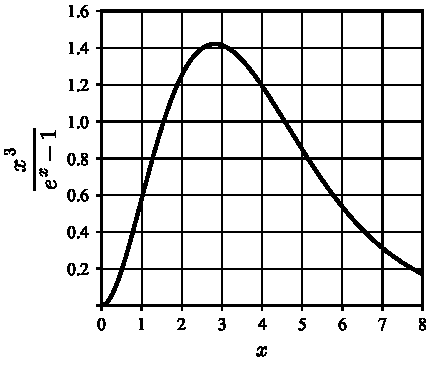
\includegraphics[width=7cm]{fig7.pdf}\\[0.3em]{\small 图 7}\end{minipage}\par\nopagebreak

黑体辐射能量的频谱分布密度 $\dfrac{\mathrm{d}E_\omega}{\mathrm{d}\omega}$ 在 $\omega=\omega_m$ 的频率处具有极大值，$\omega_m$ 由下式决定：
\begin{equation}
  \frac{\hbar\omega_m}{T}=2.822.
\end{equation}
由此可见，当温度升高时，分布的极大值的位置以与 $T$ 成正比的方式向频率较大的方向移动\footnote{按波长的分布密度 $\dfrac{\mathrm{d}E_\lambda}{\mathrm{d}\lambda}$ 也具有极大值，它的位置由另一个类似的比值
\begin{equation*}
  \frac{2\pi\hbar c}{T\lambda_m}=4.965
\end{equation*}
所决定. 由此可见，按波长的分布极大值点（$\lambda_m$）以与温度成反比的方式移动.}（维恩位移定律）.

我们来计算黑体辐射的热力学量.当 $\mu=0$ 时自由能 $F$ 同 $\Omega$ 一致（因为 $F=\varPhi-PV=N\mu+\Omega$）.根据公式(54.4)，在其中令 $\mu=0$，并且像通常那样（借助于(63.3)）从求和转换到积分，我们就得到：
\begin{equation}
  F=T\,\frac{V}{\pi^2c^3}\int_0^{\infty}
  \omega^2\ln\left(1-\mathrm{e}^{-\hbar\omega/T}\right)\mathrm{d}\omega.
\end{equation}
引入积分变量 $x=\dfrac{\hbar\omega}{T}$ 并进行分部积分，我们得到：
\begin{equation*}
  F=-V\,\frac{T^4}{3\pi^2\hbar^3c^3}\int_0^{\infty}
  \frac{x^3\,\mathrm{d}x}{\mathrm{e}^x-1}.
\end{equation*}
上式中的积分等于 $\dfrac{\pi^4}{15}$（参看§58第二个脚注）.由此可见，
\begin{equation}
  F=-V\frac{\pi^2T^4}{45(\hbar c)^3}=-\frac{4\sigma}{3c}\,VT^4.
\end{equation}
如果 $T$ 用开尔文量度，那么系数 $\sigma$ 等于
\begin{equation}
  \sigma=\frac{\pi^2k^4}{60\hbar^3c^2}=5.67\times10^{-5}\,
  \frac{\mathrm{g}}{\mathrm{s}^3\cdot\mathrm{K}^4}
\end{equation}
称为斯特藩—玻尔兹曼常量.

熵为
\begin{equation}
  S=-\frac{\partial F}{\partial T}=\frac{16\sigma}{3c}\,VT^3.
\end{equation}
它与温度的立方成正比.辐射总能量 $E=F+TS$ 等于
\begin{equation}
  E=\frac{4\sigma}{c}\,VT^4=-3F.
\end{equation}
当然，这个表达式也可以由直接对分布(63.5)积分而得到.由此可见，黑体辐射的总能量与温度的四次方成正比（玻尔兹曼定律）.

对于辐射的热容，有
\begin{equation}
  C_v=\left(\frac{\partial E}{\partial T}\right)_V
  =\frac{16\sigma}{c}\,T^3V.
\end{equation}
最后，压强等于
\begin{equation}
  P=-\left(\frac{\partial F}{\partial V}\right)_T=\frac{4\sigma}{3c}\,T^4,
\end{equation}
\begin{equation}
  PV=\frac{E}{3}.
\end{equation}
理所当然，对于光子气体可以得到与超相对论性电子气（§61）同样的压强极限表达式；关系式(63.17)是粒子的能量和动量之间的线性关系（$\varepsilon=cp$）的直接结果.

黑体辐射中的光子总数为
\begin{equation*}
  N=\frac{V}{\pi^2c^3}\int_0^{\infty}
  \frac{\omega^2\,\mathrm{d}\omega}{\mathrm{e}^{\hbar\omega/T}-1}
  =\frac{VT^3}{\pi^2c^3\hbar^3}\int_0^{\infty}
  \frac{x^2\,\mathrm{d}x}{\mathrm{e}^x-1}.
\end{equation*}
上式中的积分可以用 $\zeta(3)$ 来表示（参看§58第二个脚注）. 由此可见，
\begin{equation}
  N=\frac{2\zeta(3)}{\pi^2}\left(\frac{T}{\hbar c}\right)^3V
  =0.244\left(\frac{T}{\hbar c}\right)^3V.
\end{equation}
当光子气体做绝热膨胀（或压缩）时，体积和温度彼此由 $VT^3=$常数 的关系式联系着.同时由于(63.16)，压强和体积由 $PV^{4/3}=$常数 的关系式联系着.与(61.8)相比较，我们看到：光子气体的绝热曲线方程同超相对论性电子气的绝热曲线方程一致（这正是我们所预期的）.

我们来研究与周围的黑体辐射处于热平衡的任何物体.物体不断地反射和吸收投射到它上面的光子，同时物体本身也辐射出新的光子，并且在平衡状态下所有这些过程相互抵消，以使得光子按频率和方向的分布平均地来讲保持不变.

由于黑体辐射是完全各向同性的，能流从它的每个体积元中均匀地向四面八方流出.我们引入符号
\begin{equation}
  e_0(\omega)=\frac{1}{4\pi V}\,\frac{\mathrm{d}E_\omega}{\mathrm{d}\omega}
  =\frac{\hbar\omega^3}{4\pi^3c^3\left(\mathrm{e}^{\hbar\omega/T}-1\right)}
\end{equation}
代表在单位体积和单位立体角内黑体辐射的能谱密度.于是，从每一点流出而进入立体角元 $\mathrm{d}o$ 且频率在间隔 $\mathrm{d}\omega$ 内的能流密度为：
\begin{equation*}
  c\,e_0(\omega)\,\mathrm{d}o\,\mathrm{d}\omega.
\end{equation*}
因此在单位时间内，投射到物体表面的单位面积上而投射方向与表面法线成 $\theta$ 角（同时频率在 $\mathrm{d}\omega$ 内）的辐射能量为
\begin{equation*}
  c\,e_0(\omega)\cos\theta\,\mathrm{d}o\,\mathrm{d}\omega,\qquad
  \mathrm{d}o=2\pi\sin\theta\,\mathrm{d}\theta.
\end{equation*}
我们用 $A(\omega,\theta)$ 来代表物体的吸收本领，它是辐射频率及其投射方向的函数；这个量被定义为：投射到物体表面上的在给定频率间隔 $\mathrm{d}\omega$ 内的辐射能量被该物体所吸收的部分，不包括透过物体的辐射（如果有的话）.于是（在 $1\,\mathrm{s}$ 内、在 $1\,\mathrm{cm}^2$ 表面上）被吸收辐射的量为：
\begin{equation}
  c\,e_0(\omega)A(\omega,\theta)\cos\theta\,\mathrm{d}o\,\mathrm{d}\omega.
\end{equation}
我们假定物体不散射辐射，也不发荧光，也就是说反射时不改变 $\theta$ 角和频率.此外，我们认为辐射不能穿透物体；换句话说，所有未被反射的辐射完全被吸收了.这时被吸收辐射的数量(63.20)应该被物体本身在同一个方向上和在同一个频率间隔内所发射的辐射所抵消.用 $J(\omega,\theta)\,\mathrm{d}\omega\,\mathrm{d}o$ 来代表（从 $1\,\mathrm{cm}^2$ 表面上）发射出来的强度，并且令它等于被吸收的能量，我们就得到如下关系式：
\begin{equation}
  J(\omega,\theta)=c\,e_0(\omega)A(\omega,\theta)\cos\theta.
\end{equation}
当然，函数 $J(\omega,\theta)$ 和 $A(\omega,\theta)$ 对于不同的物体是不同的.但是，我们看到：它们的比值是频率和方向的普适函数而与物体的性质无关：
\begin{equation*}
  \frac{J(\omega,\theta)}{A(\omega,\theta)}=c\,e_0(\omega)\cos\theta,
\end{equation*}
这个函数由黑体辐射（当温度等于物体的温度时）的能谱分布所决定；这个结论就是所谓基尔霍夫定律的内容.

如果物体对光散射，那么基尔霍夫定律只能以一种更为局限的方式来表述.因为在这种情形下反射时会改变 $\theta$ 角，所以从平衡条件出发只能要求：物体从所有方向吸收来的辐射（在一定的频率下）等于物体发射到所有方向去的总辐射：
\begin{equation}
  \int J(\omega,\theta)\,\mathrm{d}o
  =c\,e_0(\omega)\int A(\omega,\theta)\cos\theta\,\mathrm{d}o.
\end{equation}
在辐射可以穿透物体的情形下，一般来讲，$\theta$ 角也发生改变（由于射入物体和由物体射出时发生折射所致）. 在这种情形下，关系式(63.22)还应该对物体的整个表面进行积分；同时函数 $A(\omega,\theta)$ 和 $J(\omega,\theta)$ 不但与物体的材料和形状有关，而且还与物体表面上的所在点有关.

最后，当有伴随着频率改变的散射（荧光）存在时，基尔霍夫定律只有在既对方向进行积分，又对辐射频率进行积分后才能成立：
\begin{equation}
  \iint J(\omega,\theta)\,\mathrm{d}o\,\mathrm{d}\omega
  =c\iint e_0(\omega)A(\omega,\theta)\cos\theta\,\mathrm{d}o\,\mathrm{d}\omega.
\end{equation}
如果一个物体能够完全吸收投射到它上面的全部辐射，那么这个物体就称为绝对黑体\footnote{这样的物体可以用空腔的形式实现，它有强吸收的内壁并备有一小孔. 从外部射入这个小孔的任何射线只有在受到腔壁的多次反射以后，才可能重新射到这个小孔上而外逸. 因此只要孔径足够小，空腔实际上把投射到小孔上的所有辐射都吸收掉，因而小孔成为绝对黑体.}.根据定义，这种物体的 $A(\omega,\theta)=1$，而它的发射本领完全决定于函数
\begin{equation}
  J_0(\omega,\theta)=c\,e_0(\omega)\cos\theta,
\end{equation}
这个函数对于所有的绝对黑体来讲都是相同的.应当注意：绝对黑体的发射强度对方向的依赖关系非常简单——它正比于发射方向同物体表面法线的夹角的余弦.把(63.24)对所有的频率和对半球内的所有立体角进行积分，就得到绝对黑体的总发射强度 $J_0$
\begin{equation*}
  J_0=c\int_0^{\infty}e_0(\omega)\,\mathrm{d}\omega\cdot
  \int_0^{\pi/2}2\pi\cos\theta\sin\theta\,\mathrm{d}\theta=\frac{cE}{4V},
\end{equation*}
式中 $E$ 由公式(63.14)所确定. 由此可见，
\begin{equation}
  J_0=\sigma T^4,
\end{equation}
即绝对黑体的总发射强度与它的温度的四次方成正比.

最后，我们来研究不处于热平衡的辐射；这种不平衡既可以指辐射谱分布，也可以指辐射按方向的分布.设 $e(\omega,\boldsymbol{n})\,\mathrm{d}\omega\,\mathrm{d}o$ 是频率在间隔 $\mathrm{d}\omega$ 内而波矢方向 $\boldsymbol{n}$ 在立体角元 $\mathrm{d}o$ 内的这种辐射的空间密度.在频率和方向的每一个小间隔内可以这样来引入辐射温度的概念：密度 $e(\omega,\boldsymbol{n})$ 等于由普朗克公式在这个温度下所给出的值，即
\begin{equation*}
  e(\omega,\boldsymbol{n})=e_0(\omega).
\end{equation*}
把这个温度表示为 $T_{\omega n}$，我们有：
\begin{equation}
  T_{\omega n}=\frac{\hbar\omega}
  {\ln\left[1+\dfrac{\hbar\omega^3}{4\pi^3c^3}\,
  \dfrac{1}{e(\omega,\boldsymbol{n})}\right]}.
\end{equation}
我们来设想一个向周围（真空）空间辐射的绝对黑体.辐射沿着直的射线自由地传播，并且在物体以外不再处于热平衡状态——它不再像平衡辐射那样是各向同性的.因为光子在真空中传播时彼此并不相互作用，所以我们有理由把刘维尔定理严格地应用于光子在它们的相空间内的分布函数，即光子按坐标和波矢分量的分布函数\footnote{在研究几何光学的极限情形时，我们可以说光子的坐标.}.根据这个定理，分布函数沿着相轨道保持不变.然而，除了一个与频率有关的因子以外，分布函数是同给定频率和方向的辐射的空间密度 $e(\omega,\boldsymbol{n},\boldsymbol{r})$ 一致的.因为辐射频率在传播时也不改变，所以我们可以有以下重要结果：在每一个有辐射在其中（从空间给定的一点）传播的立体角元中，辐射密度 $e(\omega,\boldsymbol{n},\boldsymbol{r})$ 等于在辐射黑体内部所具有的密度，也就是说等于黑体辐射的密度 $e_0(\omega)$.但是，在平衡的辐射中这样的密度是在所有的方向都存在的，而在这里这样的密度只在某个选定的方向间隔内才存在.

根据(63.26)来定义非平衡辐射的温度时，我们可以把这个结果表示为另一种形式，譬如说，对于所有的有辐射在其中（从空间的每一给定点）传播的方向来讲，温度 $T_{\omega n}$ 等于辐射黑体的温度 $T$.如果辐射温度按照对所有方向求平均的密度来定义，那么这个温度当然是低于黑体温度的.

刘维尔定理的所有这些结论在有反射镜和折射透镜存在的情形中也完全保持有效——当然是在保持几何光学适用的条件下.利用透镜或镜子可以使辐射聚焦，即扩大射线（到达空间中给定的一点）的通行方向的范围.从而可以提高在这一点的辐射平均温度；但是，由上述讨论可以得出结论：无论用什么方式也不能使它高于发射这个辐射的黑体的温度.
